%
% $RCSfile: model_driven_architecture.tex,v $
%
% Copyright (C) 2002-2008. Christian Heller.
%
% Permission is granted to copy, distribute and/or modify this document
% under the terms of the GNU Free Documentation License, Version 1.1 or
% any later version published by the Free Software Foundation; with no
% Invariant Sections, with no Front-Cover Texts and with no Back-Cover
% Texts. A copy of the license is included in the section entitled
% "GNU Free Documentation License".
%
% http://www.cybop.net
% - Cybernetics Oriented Programming -
%
% http://www.resmedicinae.org
% - Information in Medicine -
%
% Version: $Revision: 1.1 $ $Date: 2008-08-19 20:41:07 $ $Author: christian $
% Authors: Christian Heller <christian.heller@tuxtax.de>
%

\subsection{Model Driven Architecture}
\label{model_driven_architecture_heading}
\index{Model Driven Architecture}
\index{MDA}
\index{Object Management Group}
\index{OMG}
\index{Unified Modeling Language}
\index{UML}
\index{Meta Object Facility}
\index{MOF}
\index{Interface Definition Language}
\index{IDL}
\index{XML Metadata Interchange}
\index{XMI}
\index{Extensible Markup Language}
\index{XML}
\index{Common Warehouse Metamodel}
\index{CWM}
\index{Common Object Request Broker Architecture}
\index{CORBA}
\index{Platform Independent Model}
\index{PIM}
\index{Platform Specific Model}
\index{PSM}
\index{Computer Aided Software Engineering Tool}
\index{CASE Tool}
\index{DE}
\index{DE}
\index{DE}
\index{DE}

The \emph{Model Driven Architecture} (MDA) \cite{mda} (figure \ref{mda_figure}),
an approach to application design and implementation \cite{brown2004} specified
by the \emph{Object Management Group} (OMG), represents a suite of key
standards including:

\begin{itemize}
    \item[-] \emph{Unified Modeling Language} (UML): modelling, visualising and
        documenting the structure and behaviour of systems using graphical
        diagrams
    \item[-] \emph{Meta Object Facility} (MOF): representing and manipulating
        meta models using CORBA and its \emph{Interface Definition Language}
        (IDL); UML can be expressed in terms of MOF, which is done to generate
        XMI
    \item[-] \emph{XML Metadata Interchange} (XMI): interchanging UML
        metamodels and models using an \emph{Extensible Markup Language}
        (XML)-based format
    \item[-] \emph{Common Warehouse Metamodel} (CWM): enabling data mining
        across database boundaries at an enterprise using a complete,
        comprehensive metamodel; does for data modelling what UML does for
        application modelling
    \item[-] \emph{Common Object Request Broker Architecture} (CORBA):
        communicating using a programming language-, operating system- and
        vendor-independent middleware platform
\end{itemize}

\begin{figure}[ht]
    \begin{center}
        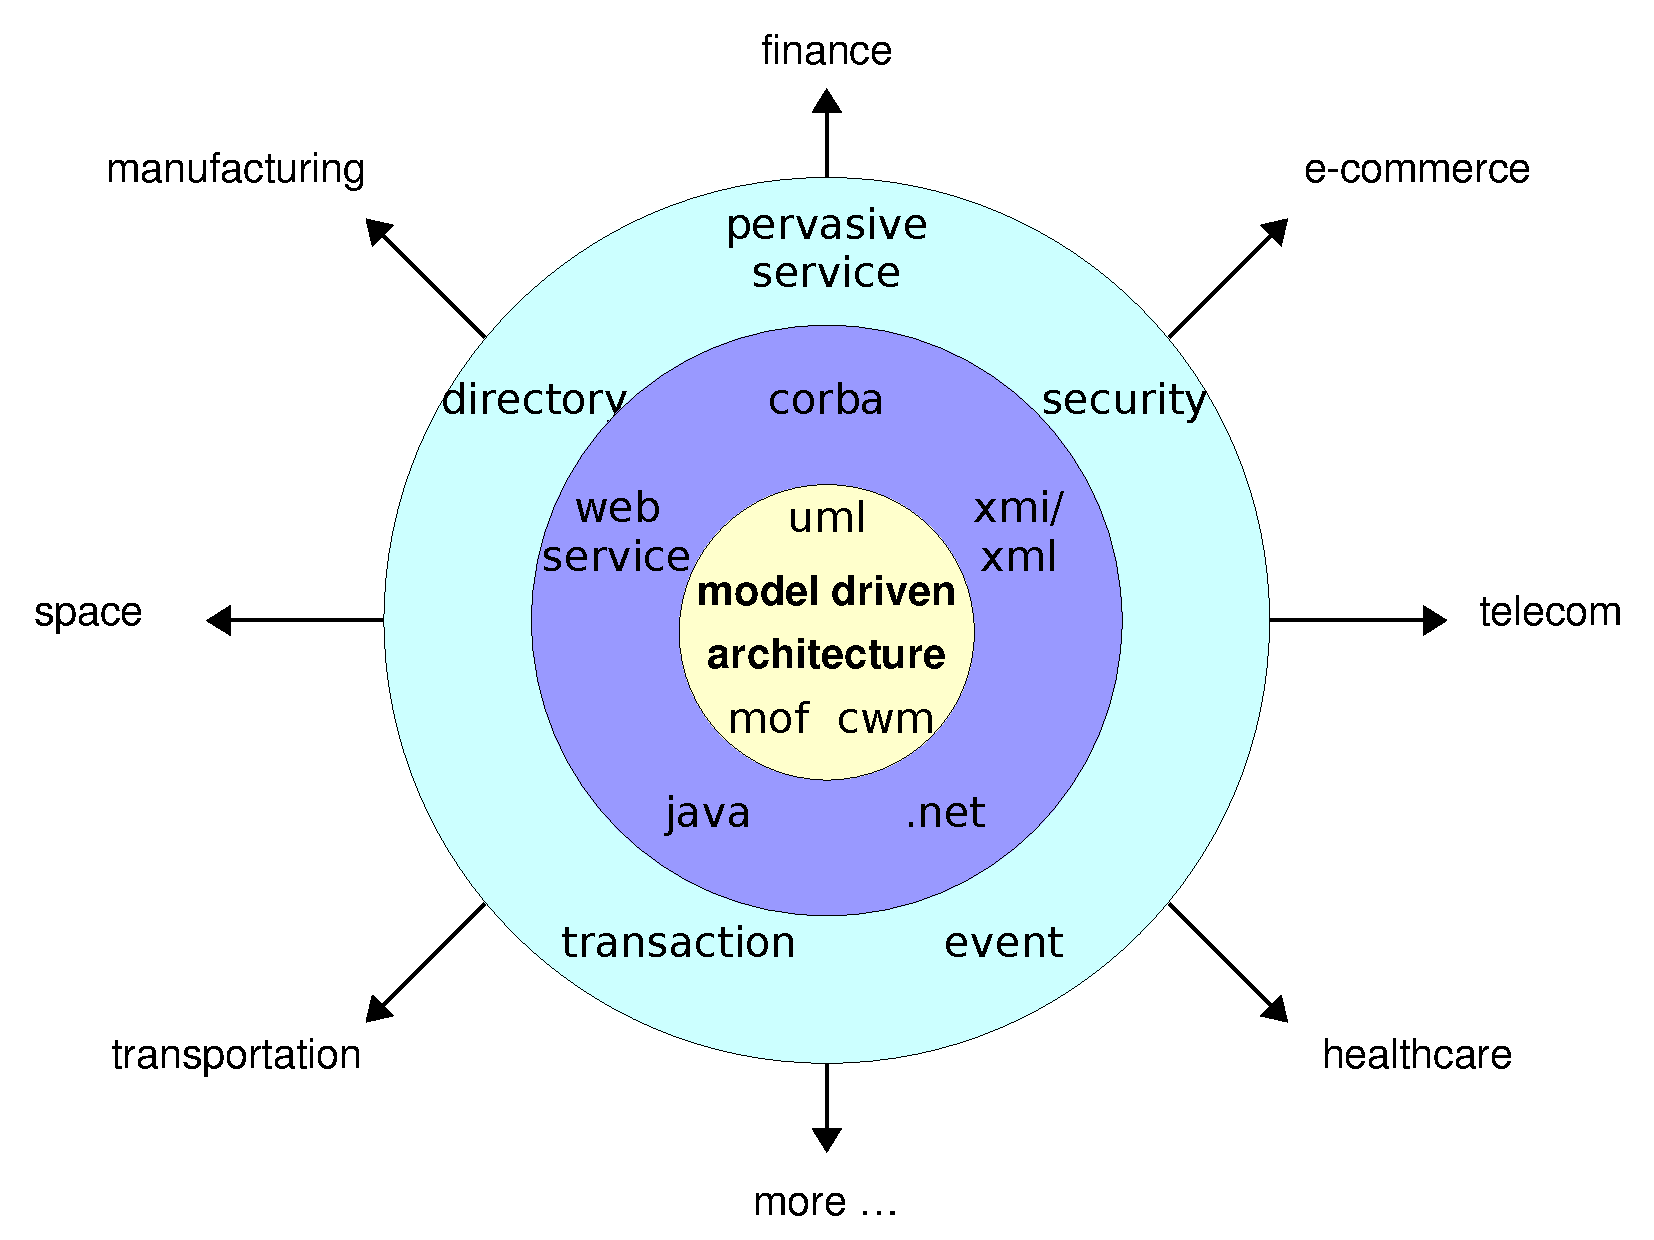
\includegraphics[scale=0.3,angle=-90]{graphic/mda.pdf}
        \caption{Model Driven Architecture \cite{mda}}
        \label{mda_figure}
    \end{center}
\end{figure}

Brown \cite{brown2004} writes: \textit{MDA encourages efficient use of system
models in the software development process, and it supports reuse of best
practices when creating families of systems.} In the OMG's own words, MDA is a:
\textit{way to organise and manage enterprise architectures supported by
automated tools and services for both defining the models and facilitating
transformations between different model types.} It aims at providing an:
\textit{open, vendor-neutral approach to the challenge of business- and
technology change}.

While traditional approaches like \emph{System Family} or
\emph{Tools \& Materials} (section \ref{tool_and_material_heading}) merely
distinguish between \emph{Domain} and \emph{Application}, the conceptual
framework provided by the MDA takes another step in separating abstract
knowledge: It treats \emph{Platform Independent Models} (PIM), that is
business- or application logic, different than the underlying
\emph{Platform Specific Models} (PSM), that is implementation technology. The
translation between the two kinds of models is normally performed using
automated tools for code generation (section \ref{generative_programming_heading}).

The MDA claims to overcome the limitations of implementation
technology-dependent \emph{Computer Aided Software Engineering} (CASE) tools
via standardised mappings and meta architectures \`a la MOF \cite{frankel}.
After Martin Fowler \cite{fowlerdsl}, one argument used in favor of MDA were
that it makes it possible to use \emph{Domain Specific Languages} (DSL)
(section \ref{domain_specific_language_heading}). However, he doubts a success
of the MDA. And indeed, although some MDA standards like the UML are very
sophisticated and widely used, it is still unclear whether the MDA, due to its
complexity, will be able to infiltrate daily software business.

But the idea of separating \emph{Application Knowledge} (PIM) from its
hardware-close \emph{Control and Processing} (PSM) clearly brings a new quality
into software development and is important for later investigations in this
work (chapter \ref{statics_and_dynamics_heading}).
